\chapter{Introduction}
Enormous datasets are a common case in today's applications. Compressing the datasets is beneficial, because they 
naturally decrease memory requirements but also are faster when compressed data is read from disk \citep{Zob95}.

One of the leading methods of data compression is variable-length coding \citep{Sal99}, where frequent sequences of data
are represented with shorter codewords. Because the sequences of data have different lengths when compressed, it is 
not trivial to determine the exact location of a certain element in the compressed data. If this is required, the usual 
data compression algorithms are inefficient. Fortunately this is not a requirement compression algorithms usually need to fulfill. However, 
random access of compressed data is useful in compressed data structures. It saves storage space, bandwith and increases the likelihood
of data already being in cache \citep{Sch02}. In most compression methods, the only way to do this is to decompress data from the beginning. 

A variable-byte encoding based integer compression method with constant time random access was first introduced by \citep{Bri09}. They used clever block 
reorganizing and $rank$ data structure to achieve random access. Their solution is currently the only published solution for the problem and it 
has been widely adopted. 

An alternative solution with $select$ data structure is proposed and explained in detail later in this thesis. Comparison to $rank$ by Brisaboa et al is shown with different
implementations of $rank$ and $select$ and several different data sets are used. Proposed method does not use data 
reorganizing, but rather capitalizes on the assumption that data is encoded the same way it is in the source. Because variable-byte encoding does not assign 
new codewords to data when encoding, reading the data straight from the memory is much faster than reassembling the word from blocks. 

(TODO: refer to results)




\chapter{Variable-byte encoding}

Variable-byte (VB) encoding \citep{Wil99} is a method for compressing integers via omitting leading zero bits that would be present in a longer fixed 
width word. In normal data sets, VB encoding loses in compression performance to generic algorithms like Huffman encoding or Lempel-Ziv encoding, but 
is generally faster to decode \citep{Bri09} and sometimes preferred due to its simplicity. As later shown in Chapter~\ref{chapter:DAC}, constant time 
random access is possible with VB encoding.

A good data set for VB encoding is a list of mostly small numbers with a need to support larger ones. A search engine may use an inverted index of 
words in documents. For each word, a list of document IDs where the word appears is stored. It may also store locations of the word in document for 
advanced search purposes. Usually these lists are preprocessed and stored as an inverted index or gaps, storing the difference to previous number 
instead of the actual number \citep{Man08}. Common words have a lot of entries in these lists, but because of gap storing the numbers are small. 
In contrast, rare words have only a few entries but the numbers stored are larger. These lists are excellent data sets for VB encoding. 

Variable-byte encoding originates from and is used in MIDI music file \citep{Mid96} and several applications have a similar implementation of VB. Apache 
Lucene has vInt datatype. Wireless Application Protocol has a variable length unsigned integer uintvar, Google Protocol Buffers has a Base 128 Varint \citep{GooPB},
 Microsoft .Net framework offers "7BitEncodedInt" in BinaryReader and BinaryWriter classes and IBM DB2 has a variable byte  \citep{Bha09}.

Elias Delta and Gamma codes \citep{Eli75} are popular encoding methods for forementioned data sets. They assign short bit array codes to small numbers, 
which allows them to outperform VB encoding on small number datasets \Citep{Wil99}. Elias Delta and Gamma codes can't support fast random access efficiently because
of their changing code length.

VB encoding splits each integer into blocks of $b$ bits and adds a continuation bit to the block to form chunks of length $1+b$. The extra bit is set to 1 only
on the block containing the least significant bits of the integer. This information is used in decoding to signal if next chunk continues the current 
integer. For example, let's assume $b = 4$ and let $n = 42$ be a 16 bit unsigned integer. The standard 8-bit representation of $n$ is 
\texttt{00000000 00101000}. When split to blocks of $b$ bits, it becomes \texttt{0000 0000 0010 1000}. Empty blocks are omitted and continuation bits 
are added to the remaining blocks. The result is \texttt{00010 11000}, which is the compressed data.

\begin{figure}[ht]
\centering
  \begin{minipage}{0.5\linewidth}
\begin{algorithmic}[H]
\Function{VBEncodeNumber}{$n$}
\State $bytes\gets $ list
\While{true}
\State \Call{prepend}{bytes,$n \bmod 128$}
\If{$n < 128$} \State break \EndIf
\State $n\gets n$ div $128$
\EndWhile
\State $bytes$[\Call{len}{$bytes$}-1] += $128$
\State \textbf{return} bytes
\EndFunction
\medskip
\medskip
\Function{VBEncode}{$numbers$}
\State $bytestream\gets $ list
\ForEach {$n \in numbers$}
\State $bytes \gets$ \Call{VBEncodeNumber}{$n$}
\State \Call{extend}{$bytestream$,$bytes$}
\EndFor
\State \textbf{return} bytestream
\EndFunction

\end{algorithmic}
\end{minipage}
\captionof{figure}{VByte encoding} \label{vbyte_enc}
\end{figure}

Decoding is essentially just reversing the encoding steps: chunks are read until a chunk with 1 as continuation bit is found. Continuation bits 
are removed from all the chunks and the blocks are concatenated to form the original number. As in the previous example, $b = 4$, encoded message 
is \texttt{00010 11000} and $n = 0$. The block from the first chunk is extracted and added to $n$, making $n = $\texttt{10}. A bitwise shift to the left 
equal to $b$ is applied to $n$, changing $n = $\texttt{100000}. Then the block is extracted from the next chunk. This block is added  $n$, making 
$n = 42$. Because the previous continuation bit was 1, decoding for this number is complete. More examples shown in Table~\ref{table:vbytes}. 
An example implementation of encode and decode with block length of 7 is shown in Figure~\ref{vbyte_enc} and Figure~\ref{vbyte_dec}.

\begin{figure}[ht]
\centering
  \begin{minipage}{0.5\linewidth}
\begin{algorithmic}[H]
\Function{VBDecode}{$bytestream$}
\State $numbers\gets $ list
\State $n\gets 0$
\ForEach {$b \in bytestream$}
\If{$b < 128$}
\State $n\gets 128\times n $ + $b$
\Else
\State $n\gets 128\times n $ + $b$ - $128$
\State $numbers$.append($n$)
\State $n\gets 0$
\EndIf
\EndFor
\State \textbf{return} numbers
\EndFunction
\end{algorithmic}
\end{minipage}
\caption{VByte decoding} \label{vbyte_dec}
\end{figure}

Small lengths of $c$ can yield better compression rate at the cost of more bit manipulation, while longer chunks need less bit manipulation and 
offer less effective compression. Generally block length of 7 has been used because it tends to perform well on average and handling chunks as bytes is 
convenient \citep{Man08}.

VB encoding is a well known compression algorithm. It's origins date back to 1980's and the famous MIDI music file format. It stored some of the numbers
in a "variable-length quantity" form, which was a 7-bit block VB structure \citep{Mid96}. Similar encoding types have existed for example in Apache Lucene 
(as vInt) and IBM DB2 database (as Variable Byte). Later, VB encoding was was to be found efficient in compressing integer lists. It was first experimented 
as a tool for compressing inverted index lists of word locations in documents \citep{Sch02}. That yielded excellent records, and since then many different 
approaches have been introduced. 

More recent studies have looked into machine code for VB and applied SIMD (Single instruction, multiple data) instructions to VB \citep{Lem18,Pla15}. The bit 
operations in VB are simple and therefore modifying the code to use SIMD instructions is straightforward and the speed improvements are significant. 

\begin{table}
\centering
\begin{tabular}{l||c c c c c} 
Original number & first block & second block & third block & fourth block &\\ 
\hline \hline 
4  & \texttt{\underline{1}4000}    &                             &                           &  &  \\
17  & \texttt{\underline{0}0001}   & \texttt{\underline{1}0001}  &                           &  &  \\
620  & \texttt{\underline{0}1100}  & \texttt{\underline{0}0110} & \texttt{\underline{1}0010} &  &  \\
60201 & \texttt{\underline{1}1001} & \texttt{\underline{0}0010} & \texttt{\underline{0}1011} & \texttt{\underline{1}1110} &  \\

\hline
\end{tabular}
\caption{VByte encoded numbers, block size 4. Continuation bit underlined.\label{table:vbytes}}
\end{table}


\chapter{Directly addressable codes} \label{chapter:DAC}

The ability to handle large amounts of data fast is one of the key challenges in the field of search engines. Compressed data structures are applied to fit the 
data into cache, memory or even hard drive. Direct access to any element in a compressed list or array is one of the usual requirements in compressed data 
strutures. It is not natively possible to decode the i-th element in variable-byte compression algorithms, because the position of the element in the compressed
list depends on the length of the preceding compressed data. Direct access is achievable with supporting data structures. A naive solution is to store the location 
of each element, but it adds a very large overhead which removes the benefit of compression.

\section{Rank and Select}
Rank and select are two succinct data structure operations which operate on a bit array B. $Rank_1$(B, i) gives the sum of 1 bits between B[0] and B[i] and 
$select_1$(B, i) gives the index of i-th 1 bit in B. Both operations can be implemented to work in constant time \citep{gbmp2014sea}. To use rank or select in indexing, the
set 1 bits in B should reflect to the element locations in the encoded data. 

For most compression algorithms, this requires B to be created in addition to the existing data and the length of B usually 
has to be close to the length of the data, because encoded element lenghts vary. VB encoding has several advantages with search and rank: the data is compressed in 
blocks of equal length which significantly shrinks the length of B. Moreover the bit array C formed from the continuation bits already stores the locations of items and works
as the needed indexing array. In this case, $rank_1$(C, i) would give the sum of end blocks up to i-th index and $select_1$(C, i) would give the location of the ending block 
of i-th compressed element.

\section{Rank and Select implementation}

The rank and select implementations used in this article are from C++ library by \citep{gbmp2014sea}. The library has several implementations of both rank and 
select as well as an implementaion of a bit array. Table~\ref{table:supportsize} has $rank$ and $select$ size requirements of implementations used in this experiment.
Both rank implementations have a constant space requirement over the bit array, while select's needed size depends on the number of 1's in the data.

The data structure of rank has two layers. First layer is the superblock array. For every 512th bit, the number of 1's from the beginning of the array is stored to the superblock array.
The second layer is the relative count block. It stores a relative count of 1's for every 64th bit. To calculate rank(i), the superblock index is s = i/512 and 
relative count block index is r = i-s / 64, both being integer divisions. Then number of 1 bits from index r to i are calculated. All three values added together add up to rank(i). 
Rankv5 is a lighter structure: it's superblock size is 2048 and relative counts are taken for every 384th bit. This causes the final bit calculation to be more costly, but reduces 
memory requirement to a quarter.

$Select$ data structure works similarly to rank. The index location of every 4096th set bit is stored in the superblock and location of every 64th set bit is stored 
relative to the superblock. With similar calculations, the location of closest 64th set bit is calculated and then bit array is iterated until required amount of bits is reached. 

In both cases, one function call always gets a value from the superblock and then from the superblock's relative block. The only differiating factor is the manual bit count from relative
block's index to wanted index. This is at most the size of one relative block and thus both of the functions work in constant time \citep{Gon05}.

\begin{table}
\centering
\caption{Memory requirements of SDSL rank and select data structures\label{table:supportsize}}
\begin{tabular}{l||c} 
Structure & Extra size taken\\ 
\hline \hline 
Rank   & \text{25\% of bit array} \\
Rankv5 & \text{6.25\% of bit array}\\
Select & \text{~8.3\% of bit array (on average)}\\
\hline
\end{tabular}
\end{table}



\section{DAC via rank}
Directly addressable codes in VB was first introduced by \citep{Bri09} in 2009. In their solution, the chunks are sorted in separate arrays by their significance. For each integer, the block 
of the least significant chunk is stored in the first array $A_1$, and its bit to the first bit array $B_1$. Then if the number was stored in multiple chunks, the block of the next chunk is
stored to $A_2$ and the bit to $B_2$ and so on. After the data is set, rank data structure is built for each bit array. Figure~\ref{bris_ds} contains a visualization of the data structure.

\begin{figure}[H]
\centering
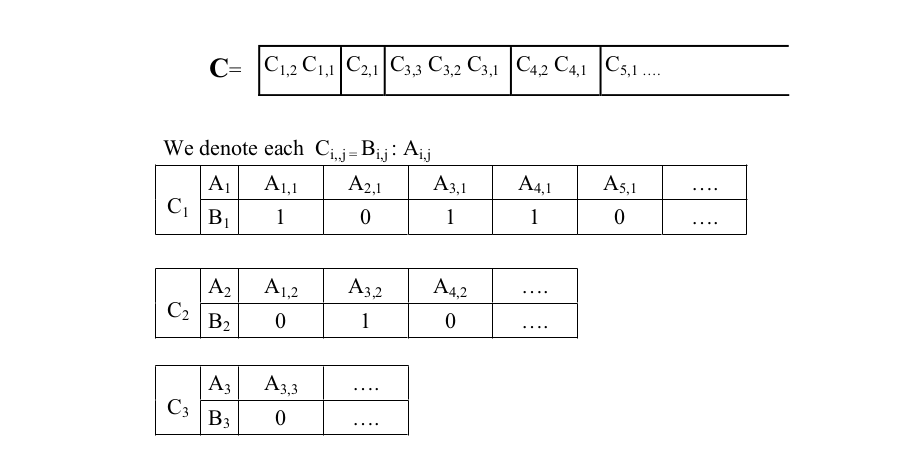
\includegraphics[scale=0.4]{bris.png}
\caption{Data structure by Brisaboa et al., visualized} (TODO: create this with tikz)\label{bris_ds}
\end{figure}

To decode an element from index i, first block is fetched from $A_1$[i]. Because each is composed of at least one block, the first block is obtainable via straight indexing. With small numbers, this 
is all that is required. If the data has a lot of small numbers, the $rank$ method has a huge advantage. However if the element was stored in multiple blocks, $i \gets rank_0$($A_1$, i) is called. $Rank_0$ 
returns the number of zeros preceding i. In other words, the number of blocks that continue to the next array. This in turn means that $i$ now has the index of the element's next block in array $A_2$.
This process is then repeated until ith bit of the current bit array is set. The decompressed integer is constructed from the fetched blocks. A pseudo code example of DAC with $rank$ is shown in Figure~\ref{bris_pseudo} 
with block length of 8.


\begin{figure}[ht]
\centering
\begin{minipage}{0.5\linewidth}
\begin{algorithmic}
\State $i \gets $ wanted index
\State $A \gets $ block arrays
\State $B \gets $ continuation bit arrays
\State $level \gets 0$
\State $number \gets 0$
\While {$B[level][index] = 0$}
\State $block \gets A[level][index]$
\State $number \gets number \mathbin{\ll} 8$
\State $number \gets number \mathbin{|} block$
\State $index \gets \Call{Rank}{B[level], index}$
\State $level \gets level + 1$
\EndWhile
\State $block \gets A[level][index]$
\State $number \gets number \mathbin{\ll} 8$
\State $number \gets number \mathbin{|} block$
\end{algorithmic}
\end{minipage}
\caption{Example pseudo code of DAC with rank by Brisaboa et al.} \label{bris_pseudo}

\end{figure}

--TODO: create another version: 7bit bris. Store bits in both bit array and chunk (to see if it's faster to get the continuation bit from the chunk than from the bit array) (also needs 7bit compliant dataset)

\chapter{DAC with select query}

Using $select_1$ on the continuation bit array to achieve direct access is more intuitive than using $rank_1$. The element locations are already marked with 1's 
in $B$ and a single $select_1$ query gets the desired starting point, while the forementioned version \citep{Bri09} used one $rank$ query for each chunk beyond 
the first. Minimizing the amount of $select$ and $rank$ queries is important. They run in constant time but their impact is huge, because rest of the VB decoding 
consists of a few bit operations. 

To use $select_1$ with VB, continuation bits need to be separated from chunks to their own bit array and a $select_1$ structure built over it. Because every compressed element has 1
only on it's last block, $Select_1$(i) returns the location of the end byte of i-th element. Therefore the start of j-th element in the block array is at 
block $b_s$ = $select_1$(j-1) + 1. Implementation was simplified by using only block sizes 4 and 8 to prevent block splitting between bytes.

Unlike the standard VB encoding, the continuation bits are removed from the chunks and stored in their own array, which leaves the blocks in their own array. This allows the 
compressed number to be read from the memory block and removes the need of block concatenation. The data in blocks is written into memory as they appear in the original integer, so that 
when reading a word from the block byte array, the bits and bytes are already in correct order. 

If the original element size is 32 bits and the data was compressed to k blocks of length b. The starting byte s of the element is $select$(i) * b div 8 where div is the integer division. 
Offset o is the remainder of previous division, o = x*b mod 8. The 32-bit word is read from memory from byte location s. Then bit shift left for 32-b*k-o is applied to remove trailing 
bits and bit shift right 32-b*k to re-align bits. If block size is one byte, offset calculation is not needed and thus the process is slightly faster.

The most intuitive way to calculate block length of i-th element is from $select_1$(i+1) and subtract the previously calculated start block index. This however causes a second 
$select_1$ query, which is costly. A much faster option is to iterate forward in bit array until the next 1. Alternatively, the block length can be calculated by reading an integer 
from the bit array, aligning it's offset and counting the trailing zeros. Figure~\ref{select_pseudo} contains an example of VB decoding with DAC with $select$ and block size 8. 
Different block sizes need extra calculation to get the block location from the byte array. In the example, $CalculateLength$ returns the length of the number in blocks and $ByteMask(k)$ returns 
a bit mask for k bytes. 

\begin{figure}[ht]
\centering
\begin{algorithmic}
\State $i \gets $ wanted index
\State $A \gets $ block byte array
\State $B \gets $ continuation bit array
\State $begin \gets \Call{Select}{index}$
\State $len \gets \Call{CalculateLength}{begin}$
\State $mask \gets \Call{ByteMask}{len}$
\State $word \gets A[begin]$ \Comment{read a word from the byte array}
\State $word \gets word \mathbin{\&} mask$ 


\end{algorithmic}
\caption{Pseudo code of DAC with select with block length 8} \label{select_pseudo}
\end{figure}

Figure~\ref{VBarrays} portrays an example of the bit array and the block array. $Select_1(k-1)$+1 returns the index of the starting byte of ith compressed element. Length of the compressed 
element is obtainable e.g. via $select_1(k)$. Then a word is read from the block array, starting from block $A_i$. Because element length in this case is 3, blocks not belonging to the element
are removed either with a bitmask or by double bit shifting, resulting in decoded k-th element.

\begin{figure}[ht]
\centering
\begin{tikzpicture}
[node distance=0pt,
 start chain = A going right,
 start chain = B going right,
 arrow/.style = {draw=#1,-{Stealth[]}, 
                shorten >=1mm, shorten <=1mm}, % styles of arrows
 arrow/.default = black,
 X/.style = {rectangle, draw,% styles of nodes in string (chain)
                minimum width=9ex, minimum height=5ex,
                outer sep=0pt, on chain}
 ]

\node[X, join] (start) {...};
\node[X] (first){0};
\node[X, very thick] (select){1};
\node[X] (Btarget){0};
\node[X, join] (second){0};
\node[X, very thick, join] (end){1};
\node[X, join] (third){0};
\node[X, join] {$B_{...}$};

\node [above=1ex of start]{Bit array};
\node [below=1ex of start]{index:};
\node [above=1ex of select]{k-1th 1};
\node [below=1ex of first]{$i-1$};
\node [below=1ex of select]{$i$};
\node [below=1ex of Btarget]{$i+1$};
\node [below=1ex of second]{$i+2$};
\node [below=1ex of end]{$i+3$};
\node [below=1ex of third]{$i+4$};
\node [above=1ex of end]{kth 1};
\node[X, below=12ex of start] (x) {...};
\node[X, join] {$A_{i-2}$};
\node[X, join] {$A_{i-1}$};
\node[X, ultra thick] (Atarget){$A_{i}$};
\node[X, ultra thick] {$A_{i+1}$};
\node[X, ultra thick] {$A_{i+2}$};
\node[X, join] {$A_{i+3}$};
\node[X, join] {$A_{...}$};
\node [above=1ex of x]{Block array};


\draw[arrow] (Btarget.south) to (Atarget.north);
\end{tikzpicture}
\caption{Data} \label{VBarrays}
\end{figure}
TODO: try bitvector SD performance + size (select) (maybe write about different select implementations)




\chapter{Experimental results}

The following experiments were run on a AMD Phenom(tm) II X6 1055T Processor@2.8Ghz with 64Kb+64Kb L1 cache, 512Kb L2 cache, 6144Kb L3 cache and 32GB of DDR3 1333MHz.
The computer runs Ubuntu 14.04.4 (3.13.0-91-generic x86\_64). The code was compiled with g++-7 -std=c++11 -DNDEBUG and with libraries -lsdsl -ldivsufsort -ldivsufsort64.

Five different VB decoding algorithms were compared. The Bris-algorithms are from \citep{Bri09}. All algorithms are implemented using data structures and functions from the SDSL 
library \citep{gbmp2014sea}. Each implementation is decoding a uint64\_t integer.

\begin{itemize}
  \item Bris4v5 - Bris implementation with block size 4, using rank support v5
  \item Bris8 - Bris implementation with block size 8, using rank support v
  \item Bris8v5 - Bris implementation with block size 8, using rank support v5
  \item Select4 - Proposed implementation with block size 4, using select support mcl
  \item Select8 - Proposed implementation with block size 8, using select support mcl
\end{itemize}






Five differently constructed datasets were used and three different sizes of dataset were used (5M, 50M, 500M). 

\begin{itemize}
  \item all - integers equally 1-4 bytes long
  \item twolarge - one eighth of integers 4 bytes long, one eighth 2 bytes long, rest 1 byte    
  \item twolarge2 - Same as twolarge, but third of the 1 byte numbers 4 bits or less
  \item onelarge - one eighth of integers 2 bytes long, rest 4 bits or less
  \item onebyte - all integers 4 bits or less
\end{itemize}

All implementation read the data set from a file and compres it to memory. Then one million index numbers are randomized to an array. The times shown in Table~\ref{table:results1} 
are times taken from looping through the index array and VB decoding the number in the index. Additionally, each run is iterated ten times and a mean of the run is taken. 

\begin{table}
\centering
\caption{Results in milliseconds, smaller is better.\label{table:results1}}
\begin{tabular}{l||c c c c c c} 
 & Bris4v5 & Select4 & Bris8 & Bris8v5 & Select8 \\ 
\hline \hline 
all (5M)        & - & 189.8 & 194.0 & 230.3 & 139.2 \\
all (50M)       & - & 292.0 & 256.0 & 304.4 & 232.7 \\
all (500M)      & - &  -    & 299.9 & 369.2 & 335.1 \\
twolarge (5M)   & - & 164.1 & 93.9  & 216.7 & 117.5 \\
twolarge (50M)  & - & 270.4 & 140.0 & 159.8 & 210.6 \\
twolarge (500M) & - & 381.4 & 169.7 & 383.6 & 307.8 \\


\hline
%
\end{tabular}
\end{table}



 - Run with 32 bit values, see what happens (some operations may be 32b?)
 - 
 - use array instead of vector<uint8 t> for bris?
- comparison to basic implementation + Bri09
  - compare with b=2,4,8

 - do we need to support search()?

 - $rank$ vs rank? should formulas have a specific style?

\chapter{Future work}
 - something to improve / research?

\chapter{Conclusions\label{chapter:conclusions}}

It is good to conclude with a summary of findings. You can also use separate chapter for discussion and future work. These details you can negotiate with your supervisor.
